\documentclass[]{book}
\usepackage{lmodern}
\usepackage{amssymb,amsmath}
\usepackage{ifxetex,ifluatex}
\usepackage{fixltx2e} % provides \textsubscript
\ifnum 0\ifxetex 1\fi\ifluatex 1\fi=0 % if pdftex
  \usepackage[T1]{fontenc}
  \usepackage[utf8]{inputenc}
\else % if luatex or xelatex
  \ifxetex
    \usepackage{mathspec}
  \else
    \usepackage{fontspec}
  \fi
  \defaultfontfeatures{Ligatures=TeX,Scale=MatchLowercase}
\fi
% use upquote if available, for straight quotes in verbatim environments
\IfFileExists{upquote.sty}{\usepackage{upquote}}{}
% use microtype if available
\IfFileExists{microtype.sty}{%
\usepackage{microtype}
\UseMicrotypeSet[protrusion]{basicmath} % disable protrusion for tt fonts
}{}
\usepackage[margin=1in]{geometry}
\usepackage{hyperref}
\hypersetup{unicode=true,
            pdftitle={Sleep quality analysis},
            pdfauthor={Arturo Laflor},
            pdfborder={0 0 0},
            breaklinks=true}
\urlstyle{same}  % don't use monospace font for urls
\usepackage{natbib}
\bibliographystyle{apalike}
\usepackage{longtable,booktabs}
\usepackage{graphicx,grffile}
\makeatletter
\def\maxwidth{\ifdim\Gin@nat@width>\linewidth\linewidth\else\Gin@nat@width\fi}
\def\maxheight{\ifdim\Gin@nat@height>\textheight\textheight\else\Gin@nat@height\fi}
\makeatother
% Scale images if necessary, so that they will not overflow the page
% margins by default, and it is still possible to overwrite the defaults
% using explicit options in \includegraphics[width, height, ...]{}
\setkeys{Gin}{width=\maxwidth,height=\maxheight,keepaspectratio}
\IfFileExists{parskip.sty}{%
\usepackage{parskip}
}{% else
\setlength{\parindent}{0pt}
\setlength{\parskip}{6pt plus 2pt minus 1pt}
}
\setlength{\emergencystretch}{3em}  % prevent overfull lines
\providecommand{\tightlist}{%
  \setlength{\itemsep}{0pt}\setlength{\parskip}{0pt}}
\setcounter{secnumdepth}{5}
% Redefines (sub)paragraphs to behave more like sections
\ifx\paragraph\undefined\else
\let\oldparagraph\paragraph
\renewcommand{\paragraph}[1]{\oldparagraph{#1}\mbox{}}
\fi
\ifx\subparagraph\undefined\else
\let\oldsubparagraph\subparagraph
\renewcommand{\subparagraph}[1]{\oldsubparagraph{#1}\mbox{}}
\fi

%%% Use protect on footnotes to avoid problems with footnotes in titles
\let\rmarkdownfootnote\footnote%
\def\footnote{\protect\rmarkdownfootnote}

%%% Change title format to be more compact
\usepackage{titling}

% Create subtitle command for use in maketitle
\newcommand{\subtitle}[1]{
  \posttitle{
    \begin{center}\large#1\end{center}
    }
}

\setlength{\droptitle}{-2em}
  \title{Sleep quality analysis}
  \pretitle{\vspace{\droptitle}\centering\huge}
  \posttitle{\par}
  \author{Arturo Laflor}
  \preauthor{\centering\large\emph}
  \postauthor{\par}
  \predate{\centering\large\emph}
  \postdate{\par}
  \date{2017-05-10}

\usepackage{booktabs}
\usepackage{amsthm}
\usepackage{multirow}
\usepackage{multicol}
\usepackage{float}
\usepackage{tabularx}
\makeatletter
\def\thm@space@setup{%
  \thm@preskip=8pt plus 2pt minus 4pt
  \thm@postskip=\thm@preskip
}
\makeatother

\begin{document}
\maketitle

{
\setcounter{tocdepth}{1}
\tableofcontents
}
\chapter{Prerequisites}\label{prerequisites}

\chapter{Introduction}\label{intro}

\hypertarget{data-adquisition}{\chapter{\texorpdfstring{\protect\hyperlink{data-adquisition}{Data
adquisition}}{Data adquisition}}\label{data-adquisition}}

\chapter{\texorpdfstring{\protect\hyperlink{data-preprocess}{Data
pre-process}}{Data pre-process}}\label{data-pre-process}

\hypertarget{feature-selection}{\chapter{\texorpdfstring{\protect\hyperlink{feature-selection}{Feature
selection}}{Feature selection}}\label{feature-selection}}

\chapter{\texorpdfstring{\protect\hyperlink{efficiency-evaluation}{Evaluation
of
Efficiency}}{Evaluation of Efficiency}}\label{evaluation-of-efficiency}

Before testing the selected factors, models were trained using the 21
sleep hygiene factors to know the predictive efficiency that these
models from various techniques of machine learning could achieve. The
result was that both, the support vector machines (SVM) with linear
kernel and logistic regression, were the two techniques with the best
results. The SVM algorithm had an efficiency of 67\% and the logistic
regression reached an efficiency of 70\%. With this background, the
tests described below were made, taking into account only the four
selected factors. If any of the techniques reaches an efficiency equal
to or higher than the previous results, the selection of variables can
be considered a successful process and these factors will be used for
the prediction model of the study hereafter.

One of the steps in the development of the investigation project,
includes the selection of a technique to train a predictive model on
supervised automated learning. We did a review of the literature and we
select three techniques under certain criterion based in the nature of
the problem. The purpose is train the model with the available data and
select the one given the best prediction. So, at the same time that the
evaluation of efficience of the selected factors was performed, the
selection of the technique that will be used for the final training was
done. The three techniques that meet the inclusion criteria, were:
artificial neural networks, vector supported machines And logistic
regression with regularization. As in feature selection, a Shiny
application was developed to process the data and compare the outcomes
for these three algorithms, training a model with total of the records
and only the four features selected in the feature selection process as
was explained in Section \ref{feature-selection}.

The evaluation was performed by the cross validation technique using an
iteration process of training, validation, analysis and refinement as
the figure \ref{fig:cross-validation-process} shows. In this process a
sixty percent of the data was used to train the model, when training
conclude, the cross validation is performed through the prediction of
the target variable in the cross validation set, containing a twenty
percent of the main dataset. The analysis is done at that time and
depending on the results, the parameters are adjusted to make a new
iteration or reach the stop point. If the stop point was reached, the
model is proved in the test set to obtain the final efficience of the
model.

\begin{figure}[H]

{\centering 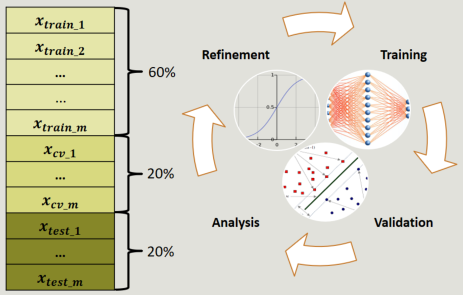
\includegraphics[width=0.8\linewidth]{images/cross-validation-process} 

}

\caption{Cross Validation Process}\label{fig:cross-validation-process}
\end{figure}

\section{\texorpdfstring{\protect\hyperlink{NN-results}{Neural Networks
Results}}{Neural Networks Results}}\label{neural-networks-results}

Two neural networks were trained and validated by cross validation
process, both estructures with a hidden layer. The first neural network
had three neurons in the hidden layer and the second four neurons. The
Fig. \ref{fig:nn-four-neurons} shows the structure of the neural network
with four neurons in the input layer, one neuron for each factor
selected in the feature selection process. The second layer is the
hidden layer with four neurons and the last layer contains one neuron
for the result (good sleep quality/bad sleep quality). Additionaly it is
possible to observe the two activation neurons in the top of the figure.

\begin{figure}[H]

{\centering 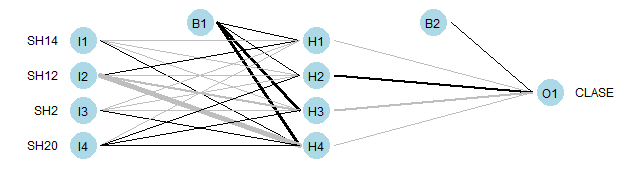
\includegraphics[width=0.8\linewidth]{images/nn-four-neurons} 

}

\caption{Structure of neural network with four neurons in the hidden layer}\label{fig:nn-four-neurons}
\end{figure}

The results for the two neural networks and the appropriate comparison
between them, are in the Fig. \ref{fig:results-of-the-3-4-nn}. The
network with better efficiency of two networks is the network with four
neurons. The table describes that in the three sets, the behavior was
superior in terms of efficiency, while the plot represents the error per
each set with three and four neurons. Clearly, the lines decrease in
favor of the training and validation with four neurons, where the error
of the prediction is smaller.

\begin{figure}[H]

{\centering 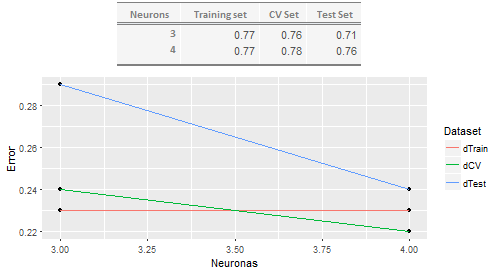
\includegraphics[width=0.8\linewidth]{images/results-of-the-3-4-nn} 

}

\caption{Comparison of the results for the two trained neural networks}\label{fig:results-of-the-3-4-nn}
\end{figure}

The results of the neural network, satisfy the conditions sought,
because although it is not greatly improved in efficiency when compared
to what can be obtained by employing all the factors of sleep hygiene,
we gain in the amount of factors that must be sensed to obtain input
data. This fact has great relevance for the project because it greatly
limits the design and infrastructure of the data acquisition module.

\section{\texorpdfstring{\protect\hyperlink{LR-results}{Logistic
Regression
Results}}{Logistic Regression Results}}\label{logistic-regression-results}

We train the model through logistic regression (LR) with regularization
parameter and polynomials of degree one, two and three, in order to look
for the optimal point between over fit and bias. The regularization
parameter based on the norm \(l_2\) takes the form of the equation
\eqref{eq:regularization-parameter}, where \(\lambda\) took values from
0.1 to 0.6 with intervals of 0.03 to choose the optimal value.

\begin{equation}
  reg=\frac{\lambda}{2m}\sum_{j=2}^{n}\theta_j^2
  \label{eq:regularization-parameter}
\end{equation}

The stop condition for the adjustment of the parameters of the
regression is of the order of one hundred thousandths, that is to say,
while the previous and the current cost function did not have a
difference of 0.00003 between both, the regression continued to iterate.

The results of LR's are shown by the application in the format of the
Fig. \ref{fig:lr-poly-1}. This figure shows the original results for the
LR with the polynomial of degree one, we obtained five coeficients
including the intercept coeficient, the right table have the data of
prediction, \(70\%\) of efficiency for the training set, \(76\%\) for
the cross validation set and \(69\%\) in the test set. The plot in the
top of figure, shows the behavior of the cost funtion through the
iterations in the compute and refinement of the parameters.

\begin{figure}[H]

{\centering 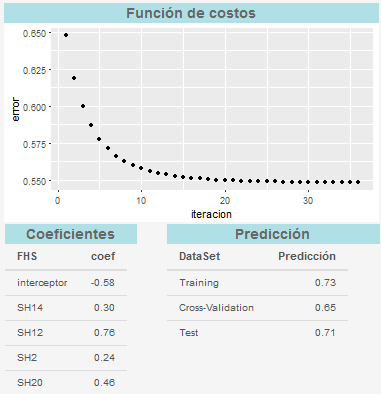
\includegraphics[width=0.8\linewidth]{images/lr-poly-1} 

}

\caption{Results of the LR and polynomial grade one}\label{fig:lr-poly-1}
\end{figure}

For polynomials of degree two and three we have a similar figure, the
difference is the number of coeficients that in the case of the
polynomial of degree two are 16 and, in the polynomial of grade three
are 35, including in both cases \emph{dummy factors}. In the case of
polynomial of degree two the cost function iterated 150 times and the
predictions were \(72\%\) of efficiency for the training set, \(78\%\)
for the cross validation set and \(69\%\) for the test set. The LR with
the polynomial of degree three, did 446 iterations, having a precision
in the prediction of \(75\%\) for the training set, \(70\%\) for the
cross validation set, falling to \(62\%\) for the test set.

\begin{table}[ht]
\centering
\caption{Comparison of efficiency of LR with polynomials of degree one, two and three}
\label{tab:results-of-efficiency-logistic-regression}
\begin{tabular}{llll}
\hline
                     & degree 1 & degree 2 & degree 3 \\ \hline
training set         & 70 \%    & 72 \%    & 75 \%    \\
cross validation set & 76 \%    & 78 \%    & 70 \%    \\
test set             & 69 \%    & 69 \%    & 62 \%    \\ \hline
\end{tabular}
\end{table}

Comparing the three results in the table
\ref{tab:results-of-efficiency-logistic-regression}, we conclude that
the polynomial of degree one is the best choice for this study, because,
is the algorithm that consumes the lower resources of the processor and
memory and have similar predictions than the other two models of degree
two and three. Results, also are satisfactory if they are compared with
the results using the 21 input data.

\section{\texorpdfstring{\protect\hyperlink{SVM-results}{Support Vector
Machine
Results}}{Support Vector Machine Results}}\label{support-vector-machine-results}

As in the previous algorithms, for support vector machines algorithm, a
cross valitation test was performed. In this case, were used four
kernels, two lineal kernels with polynomials of degree one and two, one
radial kernel and one sigmoide kernel. The Fig.
\ref{fig:SVM-sigmoide-2-flecha} shows the results as they are presnted
in the Shinny application, we can see in the left panel, the plot
showing diferents values of C and Gamma parameters and how is the
behavior of the error depending of these two parameters. In the right
side we observe that the best values for C is 0.04 and the best value
for Gamma is 0.5 to reach the best prediction for this kernel, 76\% of
prediction in the test set.

\begin{figure}[H]

{\centering 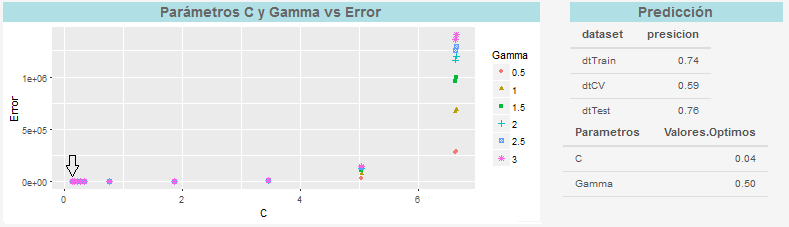
\includegraphics[width=0.8\linewidth]{images/SVM-sigmoide-2-flecha} 

}

\caption{Results of SVM with sigmoide kernel}\label{fig:SVM-sigmoide-2-flecha}
\end{figure}

The Table \ref{tab:results-of-efficiency-svm} show a comparative
framework of results of the four kernels that were tested. We can
observe that the sigmoid and radial are the best evaluated with a slight
advantage of 3 percentage points of the sigmoid over the radial. The
linear kernel is not a bad choice if one thinks in terms of simplicity
to program it and the little memory and processor that consumes.

\begin{table}[ht]
\centering
\caption{Results of officiency in prediction with SVM algorithm}
\label{tab:results-of-efficiency-svm}
\begin{tabular}{lllll}
\hline
                         & Lineal degree one & Lineal degree two & Radial & Sigmoide \\ \hline
Training dataset         & 72 \%             & 69 \%             & 80 \%  & 74 \%    \\
Cross Validation dataset & 70 \%             & 78 \%             & 69 \%  & 59 \%    \\
Test dataset             & 71 \%             & 67 \%             & 73 \%  & 76 \%    \\
Parameter C              & 0.04              & 0.14              & 0.40   & 0.04     \\
Parameter Gamma          & 0.5               & 0.5               & 0.5    & 0.5      \\ \hline
\end{tabular}
\end{table}

The Table \ref{tab:results-of-efficiency-svm}, also presents the best C
and Gamma parameters that the cross validation process selected for
these algorithm with different kernels, the parameter Gamma maintains
its value in each one of the two kernels that is required (radial and
sigmoide), 0.5 is the best value among the six values tested. On the
other hand, the parameter C, shows that small values are more
appropriate than big values. For C parameter, the best value is 0.40 for
Radial kernel and 0.04 for sigmoide kernel. C was chosen in a range of
0.01 to 1000. It means that in both cases the algorithm selected a wide
margin classifier.

\section{Comparing the results of the three algorithms and their
variants}\label{comparing-the-results-of-the-three-algorithms-and-their-variants}

All models that were trained with four factors exceed the precision of
the prediction to the models that were trained with the 21 factors
considered in the applied survey (see Table
\ref{tab:results-of-all-algoritms}). The mean of the prediction in the
models trained by the 21 factors is \(\mu=\) 63.33 with a standard
deviation of \(\sigma=\) 2.45, less than in the models trained with the
four factors selected by the algorithms described in Section
\ref{feature-selection} is \(\mu=\) 70.33 and standard deviation of
\(\sigma =\) 2.64.

\begin{table}[ht]
    \centering
    \caption{Results of all algorithms tested}
    \label{tab:results-of-all-algoritms}
    \begin{tabular}{llrrrrrr}
        \hline
        \multicolumn{1}{c}{\textbf{Algorithm}}  & \multicolumn{1}{c}{\textbf{Variant}} & \multicolumn{1}{p{1.5cm}}{\textbf{Features}} & \multicolumn{1}{c}{\textbf{Precision}} & \multicolumn{1}{p{1cm}}{\textbf{Time (sec)}} & \multicolumn{1}{p{1.5cm}}{\textbf{Features}} & \textbf{Precision} & \multicolumn{1}{p{1cm}}{\textbf{Time (sec)}} \\ \hline
        \multirow{2}{*}{ANN} & 3 Neurons    & 21  & 64\%  & 0.14   & 4  & 71\%   & 16.40   \\
                             & 4 Neurons    & 21  & 64\%  & 0.15   & 4  & 76\%   & 24.32    \\ \hline
        \multirow{3}{*}{LR}  & Linear, dg 1 & 21  & 66\%  & 0.25   & 4  & 71\%   & 0.59      \\
                             & Linear, dg 2 & 21  & 68\%  & 0.30   & 4  & 70\%   & 0.78       \\
                             & Linear, dg 3 & 21  & 60\%  & 0.70   & 4  & 64\%   & 4.44       \\ \hline
        \multirow{4}{*}{SVM} & Linear, dg 1 & 21  & 62\%  & 132.53 & 4  & 71\%   & 11.90      \\
                             & Linear, dg 2 & 21  & 62\%  & 147.21 & 4  & 69\%   & 12.46   \\
                             & Radial       & 21  & 62\%  & 20.47  & 4  & 73\%   & 8.11    \\
                             & Sigmoid      & 21  & 62\%  & 15.94  & 4  & 68\%   & 7.48   \\ \hline
    \end{tabular}
\end{table}

After obtaining these results, we decided to use only the four factors
selected to train the model for the estimation of sleep quality. The
next step is to choose the algorithm to be used for model generation.
The metrics that will be used to choose the algorithm will be, precision
of prediction, computational cost, implementation complexity in a mobile
device, and the flexibility of scaling in The time required. In the
table \ref{tab:results-of-all-algoritms}) we can see that the ANN of
four neurons and the SVM with radial kernel are the best algorithms in
prediction, however, the execution time are also of the highest. In
terms of implementation, the simplest is the LR and we can see that the
LR-trained model is below the SVM only two percentage points, and five
percentage points below the ANN Of four neurons in the hidden layer.
This allows us to have a preliminary idea of what should be done,
however it is necessary to do more tests to arrive at more solid
conclusions.

\chapter{Applications}\label{applications}

\chapter{Placeholder}\label{placeholder}

\chapter{Final Words}\label{final-words}

\bibliography{packages,book}


\end{document}
